\documentclass{article}
\usepackage{listings}
\usepackage[utf8]{inputenc}
\usepackage[spanish]{babel}
\usepackage{amsmath}
\usepackage{amsfonts}
\usepackage{amssymb}
\usepackage{graphicx}
\usepackage{lmodern}
\usepackage[left=2cm,right=2cm,top=2cm,bottom=2cm]{geometry}
\usepackage{multicol}
\usepackage{dirtytalk}
\usepackage{subfig}
\usepackage{url}
\usepackage{relsize}
\usepackage{float}

\graphicspath{ {pics/} }

\setcounter{secnumdepth}{4}
\setcounter{tocdepth}{4}

\newcommand{\parallelsum}{\mathbin{\!/\mkern-5mu/\!}}
\newcommand{\comment}[1]{}

%%CARATULA
\author{\begin{tabular}{rl}
  \textbf{Alumnos:} & Barrios Maximiliano - {149.512-4} \\ & Ebrecht Agustín {- {155.418-2} }\\ & Fritzler Pablo {- {155.413-0} }\\ & Tucci Federico{ - {149.827-7} }\\ & Videla Rodrigo{ - {146.574-0}}
\end{tabular}}


\title{{\Huge \textbf{Informe de proyecto:}}\\\vspace{10px}{Proyecto de Laboratorio}\\*
\begin{figure}[h]
\centering
\vspace{20px}

\includegraphics[width=0.6\textwidth]{UTN}
\end{figure} 
\vspace{20px}
Electrónica Aplicada III\\[0.5cm] 
\vspace{25px}
Profesor adjunto: Ing. Carlos Navarro\\
Ayudante: Ing. Alejandro Almela\\
Ayudante: Ing. Manuel Garcia Redondo
\vspace{25px}
%Ingeniería Electrónica\\
\date{\vspace{40px}CABA, Argentina, Septiembre $2019$}
}

%%%%%%%%%%%%%%%%%%%%%%%%%%%%%%%%%%%%%%%%%%%%%%%
%%ACA ARRANCA
%%%%%%%%%%%%%%%%%%%%%%%%%%%%%%%%%%%%%%%%%%%%%%%
\begin{document}

%insertar caratula
\maketitle
\thispagestyle{empty}

%insertar indice
\onecolumn
%\section{Índice}
\tableofcontents{}
\thispagestyle{empty}
\clearpage
\newpage 

%El conteo de páginas empieza aquí
\setcounter{page}{1}

%\twocolumn
\section{Introducción}

El proyecto consiste en el diseño del front-end, mostrado en la Figura 1, de un radar pasivo. Esto consiste en el cálculo de valores y elección de componentes de LNA, mezclador y topologías de filtros.

Se desea recibir una señal de RF cuya portadora es de aproximadamente de $100 MHz$ con un ancho de banda de $100 KHz$. Para ello se presenta el siguiente esquema:

\begin{figure}[H]
  \centering
    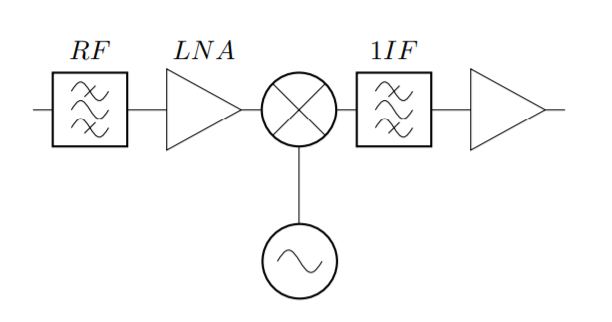
\includegraphics[scale=0.7]{esquema_circuital}
  \caption{Esquema circuital}
\end{figure}

Encaramos este diseño empleando dos circuitos integrados. El LNA lo resolveremos haciendo uso del integrado MCH4015 y para el mezclador y oscilador local usaremos el integrado SA612.

\section{Objetivos}

Nuestro primer objetivo es lograr la adaptación entre estos dos circuitos, conociendo que es de vital importancia para garantizar un óptimo funcionamiento.
 
\section{Materiales y métodos}

\comment { %%BEGIN COMENTARIO
\subsection{Front-End; \textbf{no sé si dejar esta subsección}}
El filtro de RF permitirá la atenuación de la primer frecuencia imagen que afectará al receptor superheterodino. 
\begin{center}
$f_o = 100MHz$ , $Bw = 100KHz$
\end{center}
}%% END COMENTARIO

\subsection{Primer oscilador y mezclador}
El SA612 es un circuito integrado utilizado para el procesamiento
de señales analógicas de radio. Comprende un oscilador y un mezclador. Este integrado y
frecuencias de oscilador local de hasta $200 MHz$.

Se utilizará un integrado SA612, el mismo consta de un oscilador de hasta $200MHz$ puede manejar frecuencias de señal de RF de hasta $500 MHz$. El mezclador consta de una celda de Gilbert con ganancia de $14 dB$, cifra de ruido de $5dB$ @ $45MHz$.

\begin{figure}[H]
  \centering
    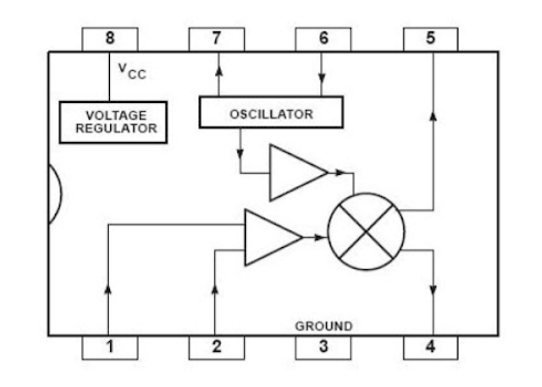
\includegraphics[scale=0.55]{SA612}
  \caption{IC SA612}
\end{figure}

La impedancia de cada entrada de CA equivalente es de aproximadamente $1.5K\Omega$ y $3 pF$ @ $50 MHz$. Cada salida es conectado a la fuente de alimentación por una resistencia interna de $1.5 K\Omega$. Esto permite tener salida balanceada, de $3 K\Omega$ y simple, de $1.5 K\Omega$.

\subsection {LNA}

Permite aumentar la potencia de señal deseada y obtener una mejora cifra de ruido del sistema cuando se lo utiliza como primer etapa (Friis), esto es, evita que el ruido sea amplificado por las etapas posteriores.
El MCH4015 es un transistor RF de bajo ruido y alta ganancia con un NF de $1.2 dB$, con una ganancia de $17 dB$.


\subsection{Procesamiento de la señal}

El procesamiento de la señal se lleva a cabo luego de la etapa del mezclador y filtros. Se opta por Red Pitaya debido a varios factores:
\begin{itemize}
    \item Es de código abierto y nos podemos nutrir de otros que ya se hayan realizado sobre esta plataforma.
    \item El costo de equipos de RF que cumplen esta función supera ampliamente al elegido.
\end{itemize}
El hardware incluye dos conversores analógico-digitales (ADC) de 125MSps y dos conversores digitales a analógicos (DAC) de 125MSps, con ancho de banda analógico de 50MHz y 14bits. Todos los puertos IO están conectados a un arreglo de compuerta programable (FPGA).
Se dispone de un sistema operativo Linux embebido, el cual es ampliamente conocido en UTN-FRBA por los docentes y alumnos de los últimos años de la carrera, lo cual permite tener un soporte para el desarrollo del proyecto. 
Dado el amplio rango de frecuencias en el cual puede trabajar Red Pitaya, podremos utilizarlo como receptor/transmisor para la banda de frecuencias que se necesita.

\begin{figure}[H]
  \centering
    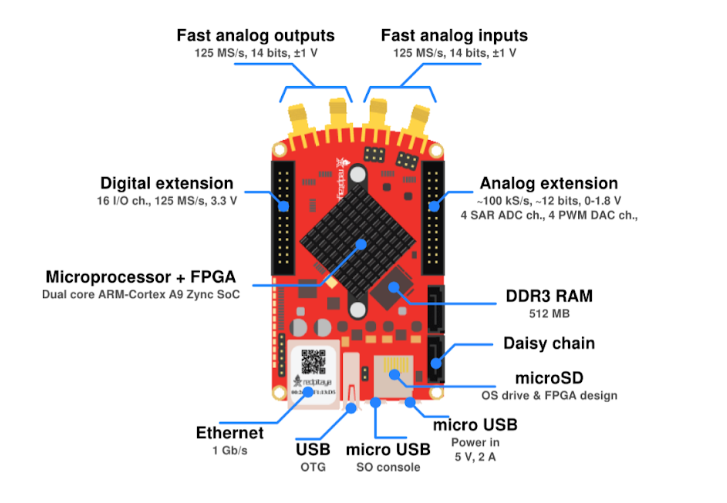
\includegraphics[scale=0.7]{PITAYA}
  \caption{ Red Pitaya }
\end{figure}

\subsection{Método utilizado}
Se analizará la impedancia que presenta el circuito de salida del transistor y se adapta con el circuito de entrada del integrado del mezclador.


Contemplamos el siguiente circuito que es la propuesta de la nota de aplicación:

\begin{figure}[H]
  \centering
    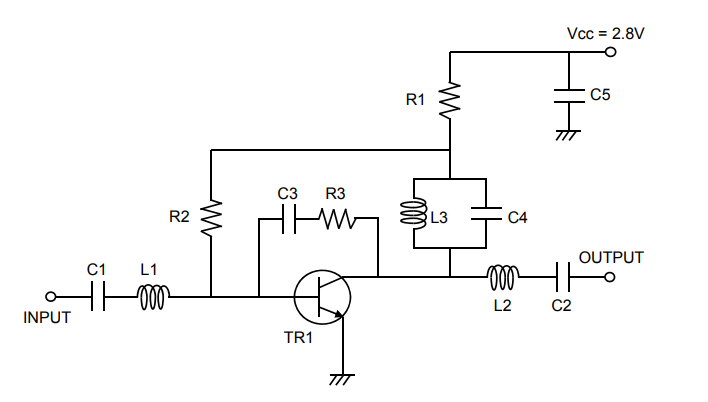
\includegraphics[scale=0.55]{ADAPT0}
  \caption{ Circuito presentado por la nota de aplicación}
\end{figure}
La impedancia, conformada por un resistor y un capacitor, que se ve a la salida de la etapa de amplificador es:

\begin{center}
    $R_{out}=900.9 \Omega$, $C_{out}=2.21pF$
\end{center}

Para la entrada del circuito del oscilador es:

\begin{center}
    $R_{in}=1500 \Omega$, $C_{in}=3pF$
\end{center}


Además eliminamos $L2$ y $C2$, y modificamos $C4$ para que el tanque resuene en $100Mhz$.

Los valores quedan:

\begin{center}
    \comment{$L2=0$, $C2=\infty$, }$L3=120nHy$, $C4=21.1pF$
\end{center}






\comment{La impedancia que se ve a la salida de la etapa de amplificador es:
$$
Z_{out}=1500 \Omega
$$
Y la que se ve a la entrada del circuito del oscilador es:
$$
Z_{in}=52 \Omega
$$
\comment{Tenemos 2 propuestas para los circuitos de adaptación.\\}
Nuestra\comment{primera} opción es una red L invertida:
\begin{figure}[H]
  \centering
    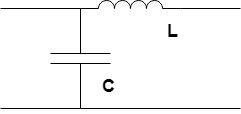
\includegraphics[scale=0.55]{ADAPT1}
  \caption{ Red L invertida }
\end{figure}
Los valores que calculamos para esta topología son:
\begin{center}
$L=27mHy$, $C=90pF$
\end{center}
\comment{
{\Large \textbf{**acá hablamos un poco del inductor elegido; johanson**}}
}
}





Proponemos la siguiente red de adaptación:

\begin{figure}[H]
  \centering
    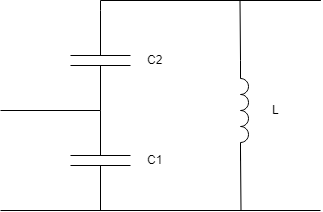
\includegraphics[scale=0.55]{ADAPT2_}
  \caption{ Red de adaptación propuesta }
\end{figure}

A ella la capacidad de salida del amplificador se le restará al capacitor $C1$, y se tendrá en cuenta también la capacidad del mezclador, la cuál se resta de las capacidades $C1$ y $C2$ en paralelo.

Los valores calculados para esta red son los siguientes:

\begin{center}
$L=120nHy$, $C1=80.89pF$, $C2=23.31pF$
\end{center}

Logrando así una adaptación entre ambos componentes.




\comment{ %% BEGIN COMENTARIO
\subsection{Adaptación de impedancias}
Es posible, en teoría, adaptar a máxima transferencia de energía y mínima cifra de ruido, sin embargo, suele no suceder lo mismo en la práctica por diversos motivos. La cifra de ruido es función de 4 parámetros para nuestro sistema :
$$
F=F_{opt} + \frac{R_{n}}{G_{s}} \cdot [ (G_{s} - G_{opt} )^{2} + ( B_{s} + B_{opt})^{2} ]
$$
El circuito de adaptación elegido para obtener esto es :
\begin{figure}[H]
  \centering
    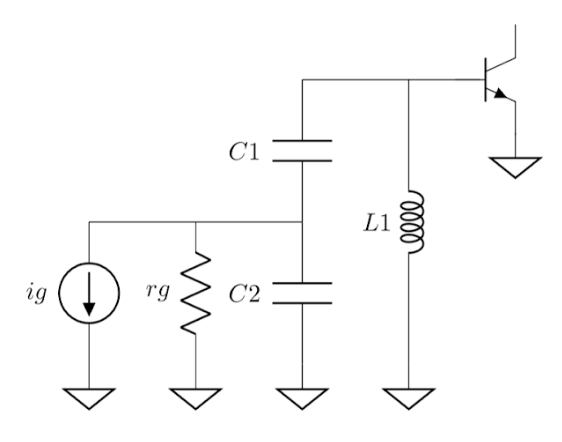
\includegraphics[scale=0.55]{ADAPT}
  \caption{  }
\end{figure}
En esta topología de celda pi capacitiva/inductiva, se pueden adaptar los niveles de impedancia vistos por el generador y por el transistor. En gran parte dependerá de los factores de calidad (Qo) de los componentes utilizados, la máxima transferencia de energía que pueda realizarse como así también el ancho de banda del filtro.\par 
\vspace{1em}
Deben considerarse también las potencias de ruido introducidas por los componentes resistivos, que para anchos de banda mayor a $1Hz$ se pueden determinar como :
$$
N_{disp} = -174dBm + 10 \cdot log(B_{Hz})
$$
Otros tipos de ruido : de disparo y Flicker (defectos en la estructura cristalina, el cual es proporcional a 1/f).
\subsection{Oscilador}
Se utilizará un oscilador controlado por tensión ( VCO ), el cual permite una estabilidad de frecuencia y un correcto control de dicha etapa.
Dado un sistema realimentado, cuando el producto de la planta y el lazo de realimentación se vuelve unitario módulo ( criterio de Barkhausen ) y el margen de fase sea cero, tenemos entonces la condición de oscilación estable.\par
Se emplea un oscilador de Colpitts cuya topología es la siguiente :
\begin{figure}[H]
  \centering
    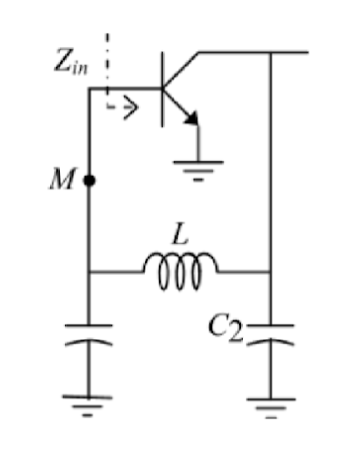
\includegraphics[scale=0.55]{COLPITTS}
  \caption{  }
\end{figure}
Entonces para la condición de Barkhausen:
$$
\alpha\beta = - g_{m} \cdot \frac{Z_{1} Z_{2}}{Z_{1} + Z + Z_{2}} = 1
$$
Donde $Z = j\omega l$ , $Z_1 = R_{transistor} \parallelsum C_1 $ y $Z_2 = 1/j\omega C_2$
\par
Para la condición de arranque :
$$
g_m \cdot r_{\pi} > \frac{C1}{C2}
$$
\subsection{Frecuencia de oscilación}
$$
\omega = \sqrt{\frac{C_2 + C_1}{C_2 C_1 L}}
$$
\subsection{Multiplicador : Celda de Gilbert}
La configuración conocida como celda de Gilbert basa su funcionamiento en circuitos pares diferenciales los cuales puede utilizarse como circuito multiplicador a partir del hecho que la corriente diferencial de salida es proporcional al producto entre la corriente de los emisores acoplados.
\begin{figure}[H]
  \centering
    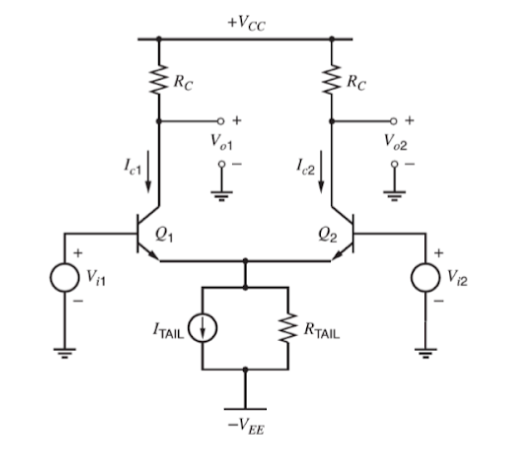
\includegraphics[scale=0.55]{GILBERT}
  \caption{  }
\end{figure}
Como se aprecia en la curva característica, el rango de tensiones en los cuales se mantiene la linealidad de respuesta es acotado y de muy baja amplitud ( se considera Vid < Vt ) . Así también es importante tener en cuenta las capacidades asociadas al amplificador, ya que la carga y descarga de las capacidades internas pueden interferir en la respuesta de las señales inyectadas y de salida.
\begin{figure}[H]
  \centering
    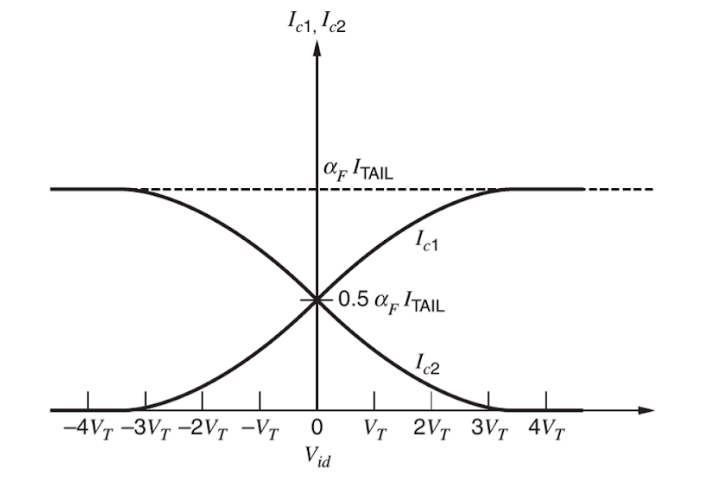
\includegraphics[scale=0.55]{RTA}
  \caption{  }
\end{figure}
\subsection{Software Defined Radio}
Es un sistema de radiocomunicaciones donde varios de los componentes típicamente implementados en hardware (mezcladores, filtros, moduladores/demoduladores, detectores, etc) son implementados en software, utilizando un ordenador personal u otros dispositivos de computación embebidos.  
Sin embargo, éste no nos exime del empleo de la etapa de front-end, donde debe hacerse el acondicionamiento de las señales para la adquisición de señales por el ADC y su posterior procesamiento. 
\begin{figure}[H]
  \centering
    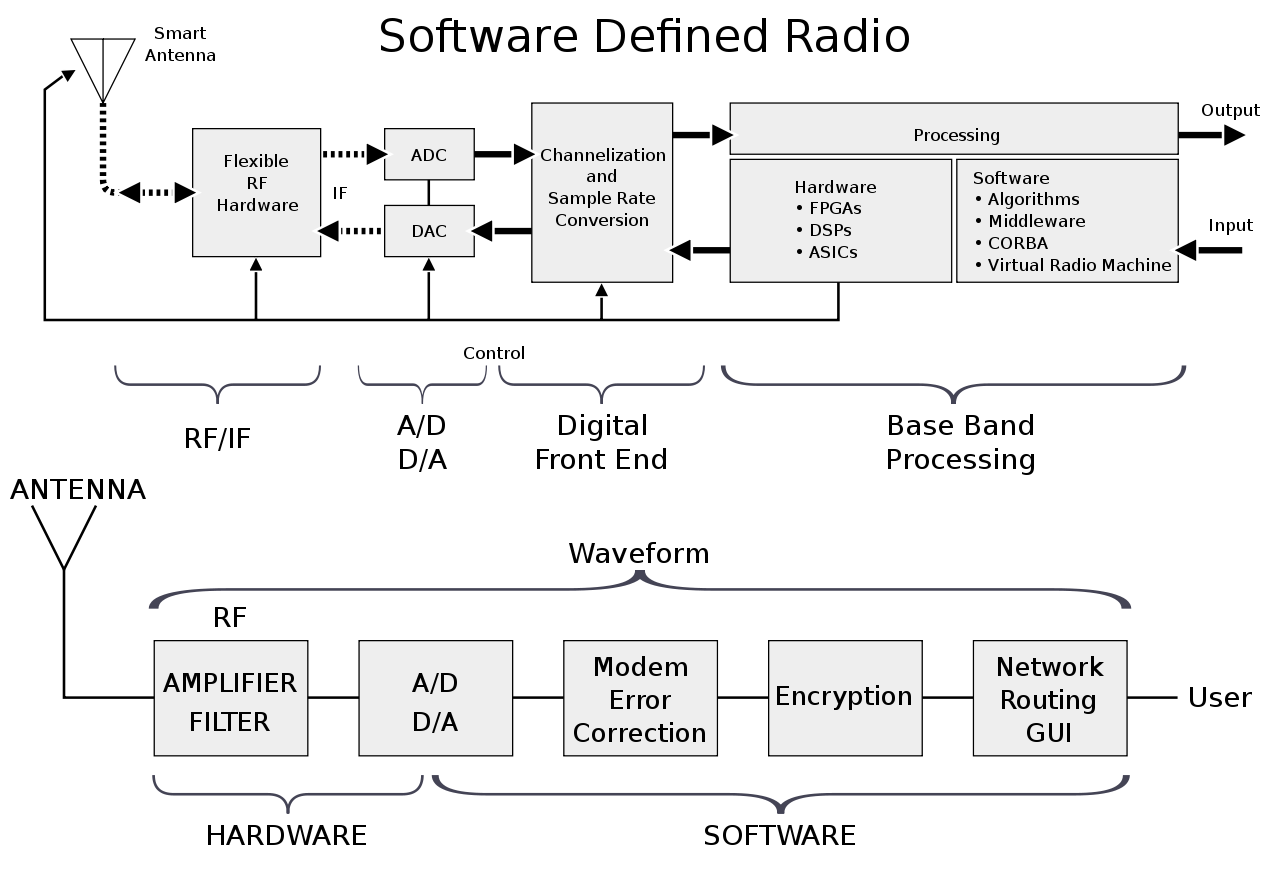
\includegraphics[scale=0.3]{SDR}
  \caption{  }
\end{figure}
}%% END COMENTARIO











\section{Conclusiones}

Esperamos poder integrar los conocimientos de la clase a este proyecto, lograr la detección de un objeto y determinar la distancia respecto al radar, utilizando lo aprendido durante la cursada e implementando los circuitos, cuyas técnicas de diseño fueran incorporadas gracias a la asignatura.
\end{document}


%% Para hacer comentarios:

\comment{ comentario }

%% también se puede usar \begin{comment}, que debe terminar con \end{comment} pero adentro del documento (\begin{document}) no compila. Acá el ejemplo (afuera del documento) con el código adentro de cómo meter una imagen


\begin{comment}

\begin{figure}[H]
  \centering
    \includegraphics[scale=0.55]{NOMBRE_SIN_EXTENSION_DE_ARCHIVO}
  \caption{  }
\end{figure}

\end{comment}